%!TEX root = ../username.tex
\chapter{Genetic Algorithms} \label{ga}

In this project, the melodies generated by the Markov model are used as the initial population for the genetic algorithm.

\section{Fitness Function} \label{ga:fitness}

Several previous papers discuss the use of interactive fitness functions \cite{papadopoulos_ai_1999, mcvicar_autoguitartab:_2015}.
With this method, a human listens to the melodies and selects the best from each generation to be used as the parents of the next generation.
This method does well at picking the most pleasing music to human ears, but it requires humans to listen to the music, which is slow and can lead to fatigue on the part of the evaluators.

Rather than rely on humans who may become tired, and may not be completely objective, we want to use an automated fitness function.
Some authors discuss techniques for fitness functions as applied to music \cite{papadopoulos_ai_1999, de_freitas_originality_2011, alfonseca_fitness_2006}.
For example, Alan de Freitas and Frederico Guimaraes use a fitness function that penalizes any note outside of the C Major scale \cite{de_freitas_originality_2011}, while George Papadopoulos and Geraint Wiggins use a fitness function that considers several characteristics of the melody, including consecutive intervals, note durations, and melodic contour \cite{papadopoulos_ai_1999}.
Music from the common practice period of Western music, which lasted from the late Baroque period through the Romantic period (1650-1900), generally followed a complex set of rules regarding harmony, rhythm, and duration.
We could manually define a function that applies some penalty for breaking one of these rules, but this approach could be highly error prone and require lots of manual tweaking.
Additionally, if we want to create music resembling a different era, we would have to write a new fitness function.
% Apparently, George Papadopoulos shares the same name as someone who plead guilty to lying to the FBI. What an unfortunate name to share.

Rather, a fitness function can be approximated using what we call a \textit{surrogate model}. % cite a paper on this
A surrogate model is used in contexts where direct measurement is computationally expensive or otherwise difficult to define.
% TODO write about accuracy results from these authors
In this project we use an artificial neural network as the surrogate model.
We expect the neural network to pick up on which rules are the most important, altering its weights accordingly.
Because music has temporal properties, the type of neural network used in this project is a \textit{long short-term memory} (LSTM) neural network.
An LSTM network is a special type of \textit{recurrent neural network}, where nodes link back to themselves.
This property of saving information about previous elements in the input sequence allows the LSTM neural network to build relationships between parts of the inputs that are far apart in a time sequence.
% TODO insert graphic here

We have two classes of training data: ``good'' melodies, which were written by a real composer, and ``bad'' melodies, which are entirely randomly generated before training the fitness function.
We expect the network might pick up on attributes such as how long a note lasts, what the pitch of a note is, and its relation to the notes around it.
Notes can be related to those around them in terms of pitch -- pitches might form a broken chord -- or in terms of rhythm -- eighth notes or sixteenth notes often appear in groups.
However, we cannot know for certain what the network decides is important before training.

In our corpus of music, the sixteenth note is most commonly the smallest rhythmic value in a piece of music, so we first preprocess the music data by converting all rhythms to consecutive sixteenth notes.
The motivation for this method, rather than trying to encode the rhythm in another way comes from Peter Todd \cite{todd_connectionist_1989}.
See Section \ref{software:ga:fitness} for more information about how the data is presented to the neural network and the configuration of the network.

During training, in addition to samples of correct music from our corpus, we also feed the network samples of random noise as incorrect examples.

Using this network setup, we regularly achieved $99\%$ accuracy determining which samples are real music and which are random notes.

A detailed description of the software implementation of the fitness function is in Section \ref{software:ga:fitness}

\section{Mutations} \label{ga:mutate}

There are several natural mutations to consider when working with music.
Two common compositional techniques are inversion and retrograde.
Inversion takes a section of music, generally a couple of measures, and inverts all the intervals, so an interval up becomes the same interval down.
Retrograde reverses the order of one or both of the rhythms and pitches of a section of music.
Retrograde and inverse can also be combined, to yield retrograde-inverse.
Typically, the section is inverted, and the new notes are then read backwards, though some composers, such as Igor Stravinsky, reversed the order of the notes first.
See Figure \ref{fig:p-r-i-ri} for an example of inversion, retrograde, and retrograde-inversion.
These techniques are especially common in twelve tone music, which was developed during the early twentieth century by Arnold Schoenberg, though they can also be found in other types of music. % TODO give examples
In our genetic algorithm, we apply these compositional techniques to the melodies from the previous generation to produce new candidates for the current generation.

\begin{figure}
	\centering
	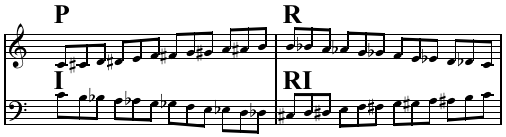
\includegraphics[width=\linewidth]{figures/P-R-I-RI.png} % TODO cite image https://commons.wikimedia.org/wiki/File:P-R-I-RI.png
	\caption{Common  clockwise from the top left: prime (original form), retrograde, inverse, and retrograde-inverse.}
	\label{fig:p-r-i-ri}
\end{figure}

An important idea when working with genetic algorithms is \textit{crossover}, where members of the population are spliced together to create new candidates.
In crossover, the fittest members of the previous generation are ``mated'' by choosing points and 
Finally, to maintain diversity in the population, we introduce some random changes to the population at a rate determined by some volatility factor, which can either stay constant or change over time.
% TODO expand on crossover

%\section{Manipulating Melodies} \label{ga:manip}


A detailed description of the genetic algorithm software is in Section \ref{software:ga}.